
\chapter{The human hearing system}
\section{Anatomy of the ear}
	\begin{wrapfigure}[12]{l}{7cm}
	\vspace{-5mm}
	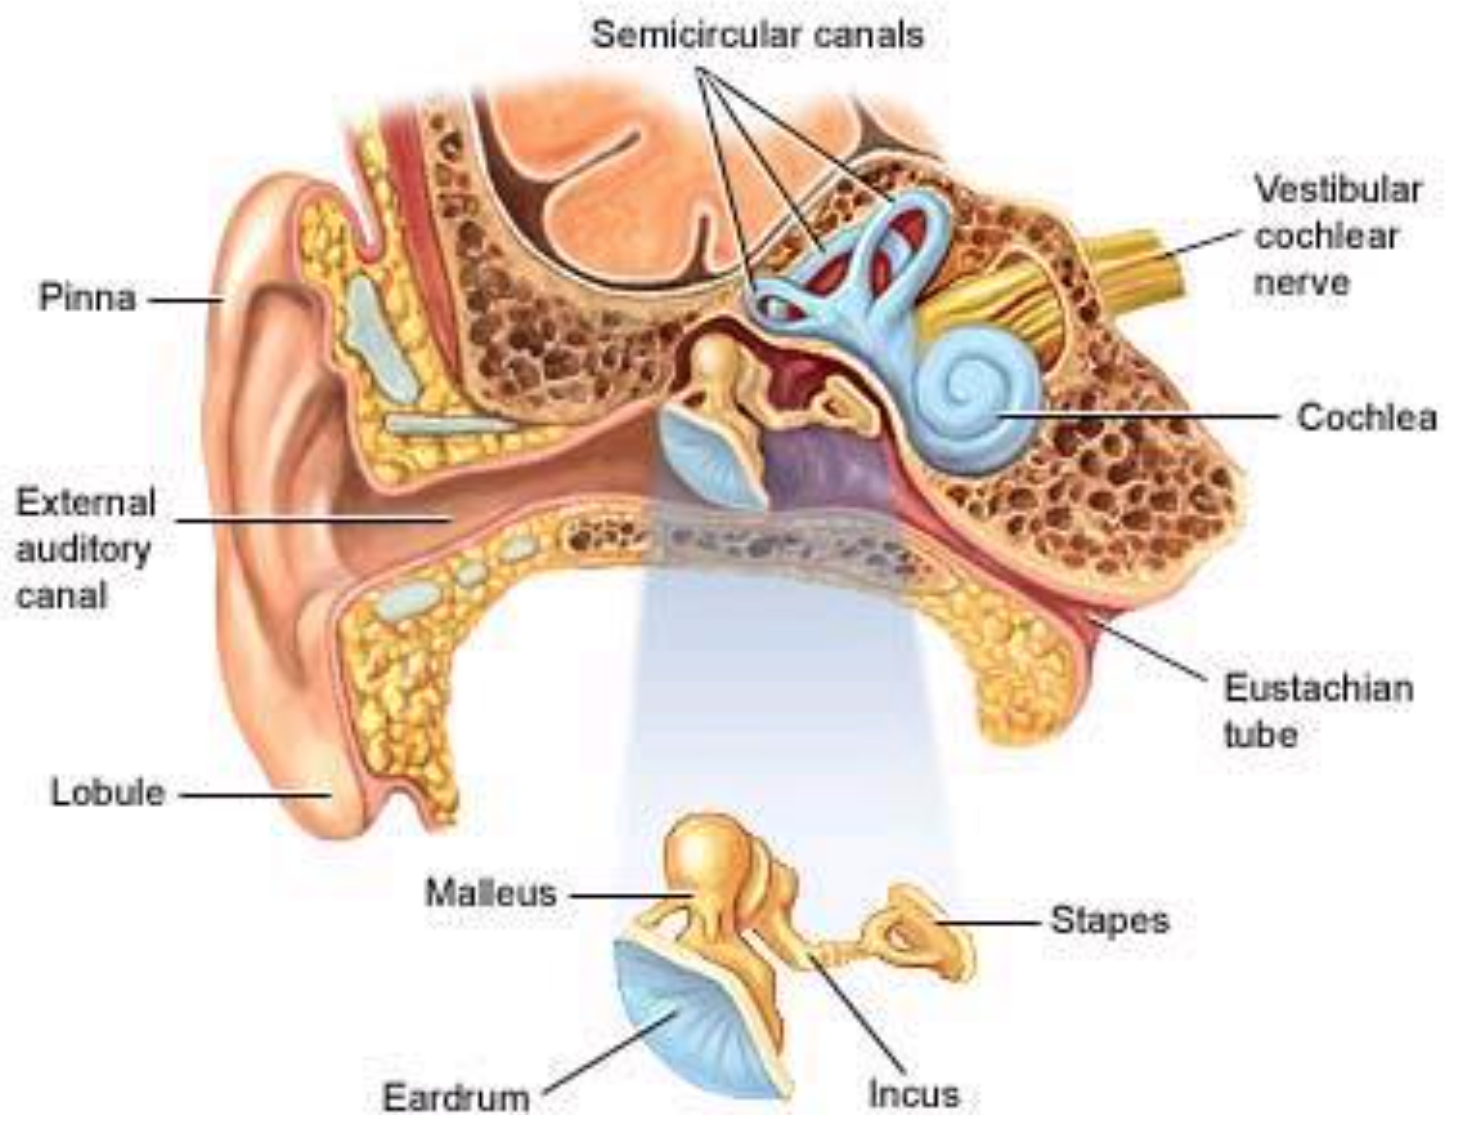
\includegraphics[scale=0.25]{acoustics/ch2/1}
	\captionof{figure}{}
	\label{fig:2.1}
	\end{wrapfigure}
	The hearing organ is sketched in \autoref{fig:2.1} and consists of three parts: the external hearing organ, the middle ear and the inner ear. The external hearing organ consists of the pinna (also called auricle), the external auditory canal and the ear drum. The middle ear consists of the hammer (malleus), anvil (incus), stirrup (stapes) and also the eardrum. The inner ear consists of the cochlea. \\
	
	The sound first comes to the auricle, then the external auditory canal which  has a 3cm length and has a resonance frequency which amplifies the sound. Then the eardrum, thin member that starts to vibrate, then we have the ear-bones that moves and transmit the vibrations to the cochlea. When a strong sound stimulant enters, a muscle attached to the stapes contracts to limit the movement of the middle ear (acoustic reflex). 
	
	\begin{wrapfigure}[12]{r}{7cm}
	\vspace{-5mm}
	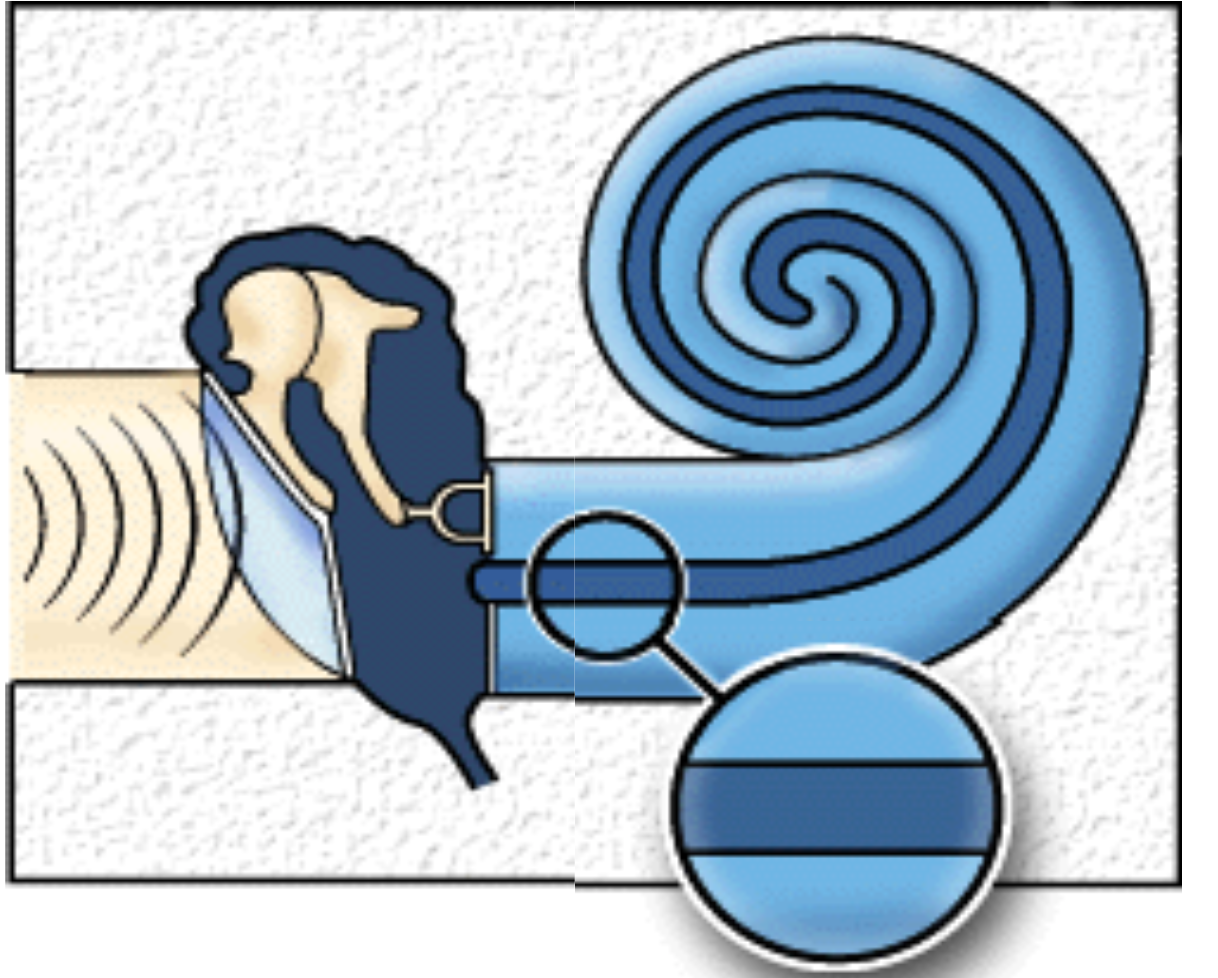
\includegraphics[scale=0.25]{acoustics/ch2/2}
	\captionof{figure}{}
	\label{fig:2.2}
	\end{wrapfigure}
	Inside the cochlea we have a liquid (the endolymph), it is divided into two tubes by the cochlear tube and are connected at the end of the spiral. When a sound comes to the eardrum, the ossicles compress the upper channel, where pressure waves propagate. We have water in the cochlea so if we don't have the bones that do the mechanism, we don't hear anything as the sound impedance is different in water and air. The transversal component of the wave exerts its force directly on the cochlear duct where the \textbf{organ of Corti is located}. 